\vspace{-2mm}
\section{Methodology}
\label{sec:methodology}
\vspace{-1mm}

\noindent\textbf{Finding a Supermask for Randomly Weighted Transformer.} 
In a general pruning framework, denote weight matrix as $\rmW\in\sR^{d\times d}$  ($\rmW$ could be a non-square matrix), input as $x\in\sR^d$ and the network as $f(x; \rmW)$. 
A subnetwork defined is $f(x; \rmW \odot \rmM)$, where $\rmM\in\sR^{d\times d}$ is a binary matrix and $\odot$ is the element-wise product. 
To find the subnetwork for a randomly weighted network, $\rmM\in\sR^{d\times d}$ is trained while $\rmW$ is kept at a random initialization. 
Following~\citet{Ramanujan:2020hidden}, denote $\rmS\in\sR^{d\times d}$ as the associated importance score matrix of $\rmW$, which is learnable during training. 
We keep top-k percents of weights by the importance score of $\rmS$ to compute $\rmM$, i.e., 
\begin{equation*}
\label{eq:topk}
\resizebox{\linewidth}{!}{$\displaystyle
% \small
\rmM = \text{Top}_k(\rmS), \text{where}
    ~\text{Top}_k(\rmS_{i, j}) = 
    \begin{cases}
    ~1 &\rmS_{i, j}\text{ in top k\%},\\
    ~0 &\text{else}.
    \end{cases}
    $
}
\end{equation*}
Note that $\text{Top}_k$ is an undifferentiated function.
To enable training of $\rmS$, we use the straight-through gradient estimator \citep{bengio2013estimating}, in which $\text{Top}_k$ is treated as the identity in backpropagation. 
During inference, we can simply construct and store the binary Supermask $\rmM$ and the floating-point $\rmW$ while dropping $\rmS$ for future usage. 

\noindent\textbf{One-layer randomly weighted Transformer.}
We use the Transformer architecture (see ~\newcite{Vaswani:2017attention} for more details).
For a general randomly weighted Transformer model with Supermask, there exist $\rmM_l$s and $\rmW_l$s for all layers $l \in \{1, ... L\}$. 
Due to the natural property of layer stacking in Transformers, all $\rmW_l$s have the same shape with the same initialization method. 
This leads to an unexplored question: ``What's hidden in a one-layer (instead of L-layer) randomly weighted transformer?''



\begin{figure*}
    \centering
    \begin{subfigure}{.4\textwidth}
        \centering
        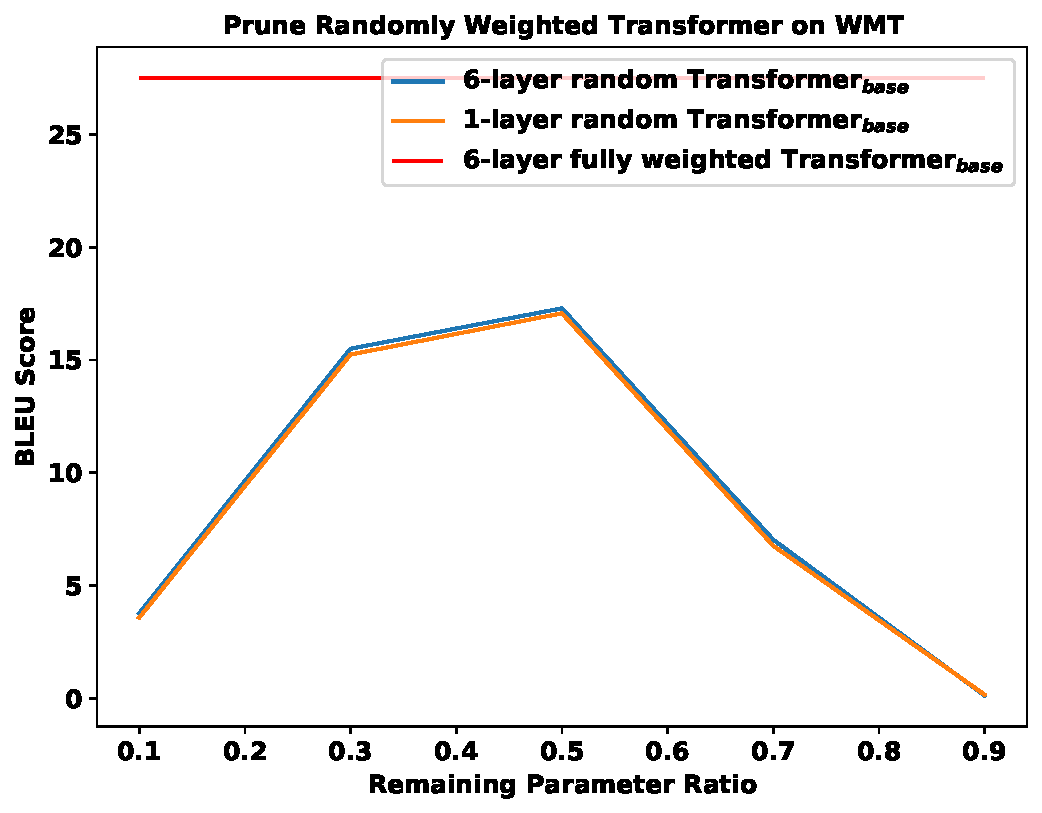
\includegraphics[width=\textwidth]{fig/wmt_result.pdf}
    \end{subfigure}%
    \begin{subfigure}{.4\textwidth}
        \centering
        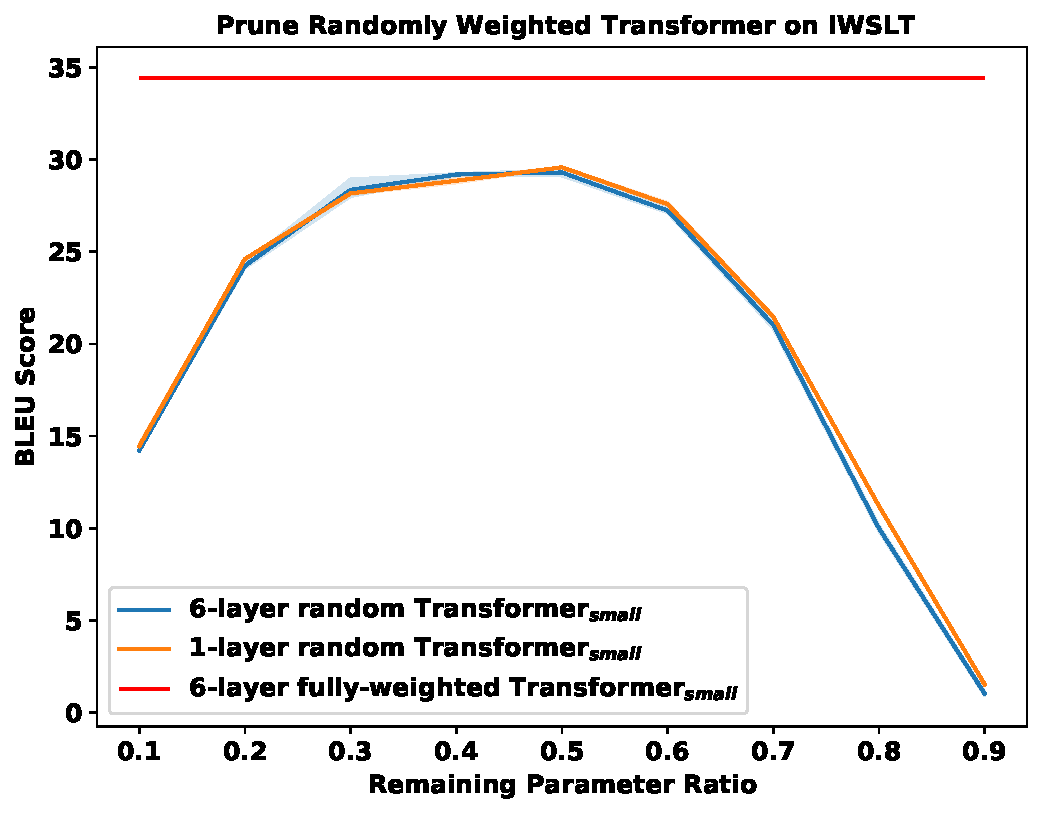
\includegraphics[width=\textwidth]{fig/iwslt_base.pdf}
    \end{subfigure}
            \vspace{-5pt}
    \caption{Prune Randomly Weighted Transformer performance on WMT14 (left) and IWSLT14 (right).}
    \label{fig:mt_base}
            \vspace{-5pt}
\end{figure*}

\begin{figure*}
    \centering
    \begin{subfigure}{.4\textwidth}
        \centering
        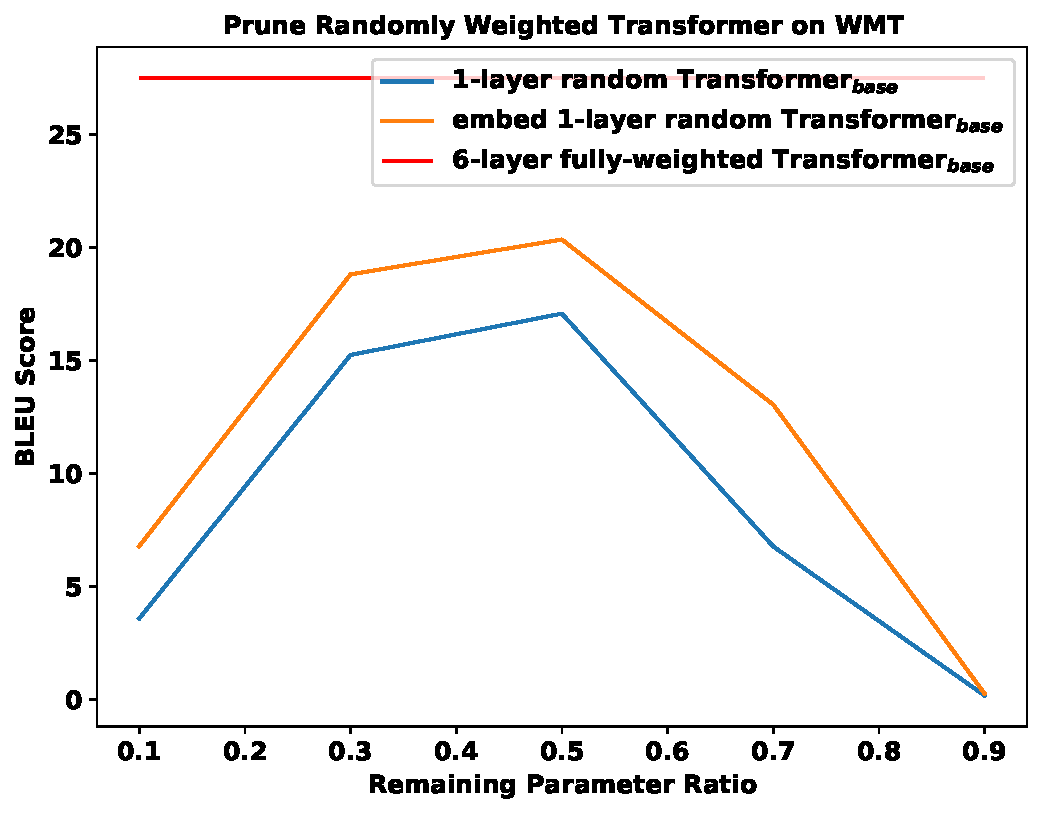
\includegraphics[width=\textwidth]{fig/wmt_embed.pdf}
    \end{subfigure}%
    \begin{subfigure}{.4\textwidth}
        \centering
        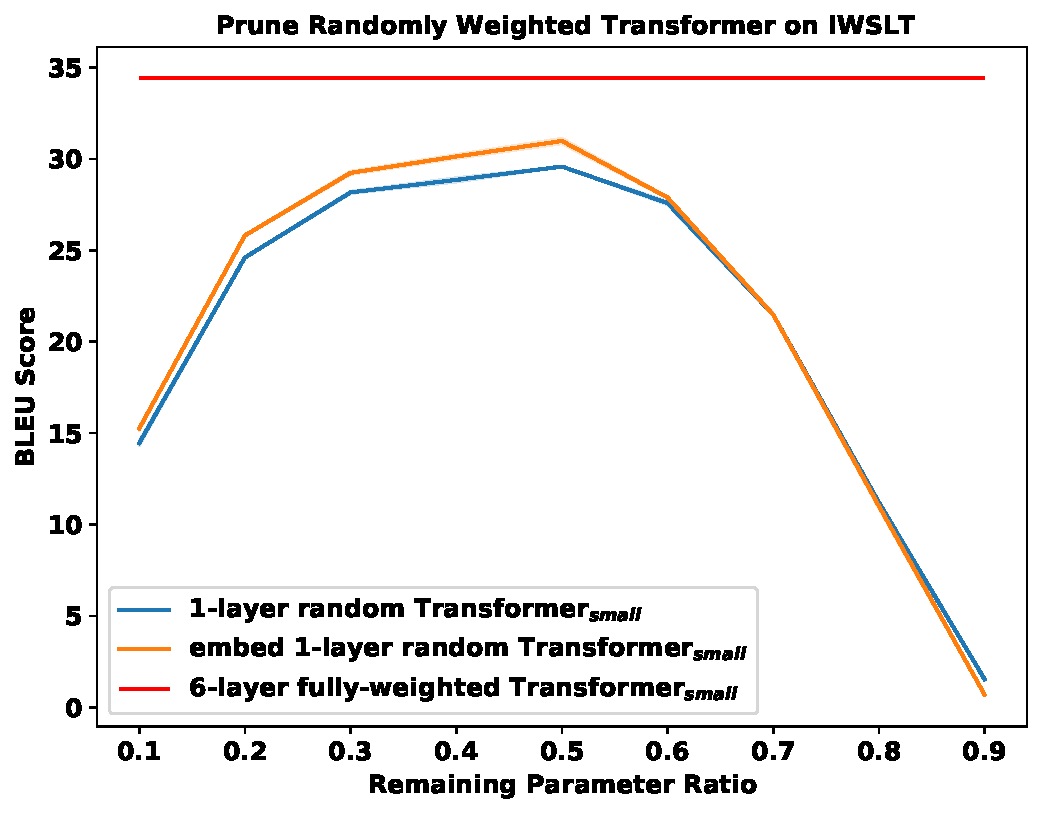
\includegraphics[width=\textwidth]{fig/iwslt_embed.pdf}
    \end{subfigure}
            \vspace{-5pt}
    \caption{The effectiveness of pre-trained embedding layers on WMT14 (left) and IWSLT14 (right).}
    \label{fig:mt_embed}
            \vspace{-10pt}

\end{figure*}

Let us use a toy example to explain why there is no need for $L$ redundant $\rmW_l$s. 
Assume that, for a random weighted matrix $\rmW_l$, the probability that it has a ``good'' subnetwork is $p$\footnote{Here, the ``good'' can be any defined metric, e.g., $(\rmM\odot\rmW_l)\text{x}\approx\rmW^*\text{x}$ for all $x$ and a pre-defined $\rmW^*$.}. 
Furthermore, assume that for two different layers, the probability that both have the ``good'' subnetworks is independent.
Then for $L$ different layers, the probability that all $\rmW_l$s have the ``good'' subnetworks is $p^L$. 
Meanwhile, since $\rmW_1$ has the same initialization method as $\rmW_l$, the probability that $\rmW_1$ has a ``good'' subnetwork for $l$-th layer is also $p$.
Thus, for $L$ different layers, the probability that using $\rmW_1$ to generate all ``good'' subnetworks is also $p^L$. 

In this paper, we investigate the scenario where one randomized layer is applied for $L$ times repeatedly with $L$ different Supermasks. 
As a result, this can reduce the memory footprint since all Supermasks can be stored in the binary format. 

